\section{Architektura IoT sítí}
  V blízké době se očekává stále větší nárůst zařízení, která jsou připojena k internetu.
  Dle odhadů by jejich počet měl v roce 2020 překročit 30 miliard \cite{iotDevices}.
  Pro takové množství připojení už není možné, aby každé zařízení komunikovalo přímo
  se vzdáleným datovým centrem, protože nároky na potřebnou šířku pásma by byly 
  obrovské \cite{fog}.
  Dalším problémem je často velmi omezený výkon připojených prvků, který je nezbytný pro 
  použití bezpečnostních funkcí umožňujících kompletně zabezpezpečenou komunikaci. 
  
  Řešení těchto problémů je do probíhající komunikace přidat několik podvrstev, 
  které umožní přesunout výpočetní výkon blíže ke koncovým zařízením, a tím celý
  proces zpracování dat provést efektivněji.
  
  V následujících podkapitolách bude popsán nový model komunikace, který přináší 
  IoT sítě.
 \subsection{Fog computing} 
 Fog computing je rozšíření Cloud computingu, které spočívá v přesunutí výpočetního
 výkonu blíže k okraji sítě. Rozšíření je umožněno pomocí přidání síťových zařízení,
 které kromě běžných funkcionalit poskytují i výpočetní výkon pro běh externích programů. Programy 
 je často možné nasadit pomocí kontejnerů nebo samostatných virtuálních strojů, což 
 velmi usnadňuje jejich distribuci \cite{fog}.
 
 Porovnání klasické a Fog architektury se nachází na obrázku \ref{obr.fog}. V reálném nasazení může
 být použito i více Fog vrstev, kde každá provádí určitý stupeň předzpracování a řízení
 dat.
\begin{figure}[ht]
\begin{center}
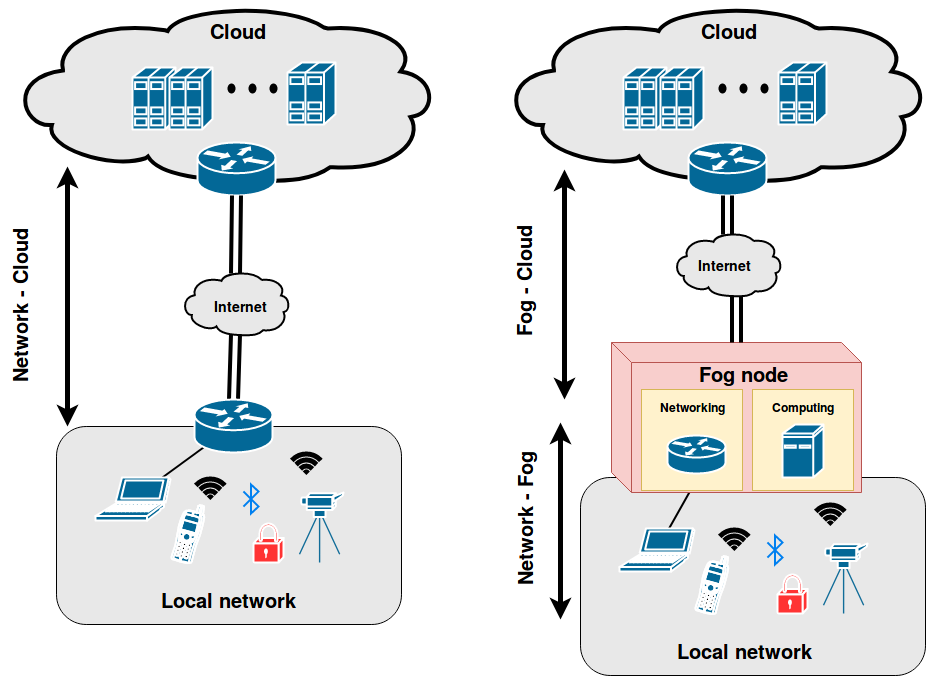
\includegraphics[scale=0.38]{pictures/fog}
\caption{Porovnání klasické a Fog architektury}
\label{obr.fog}
\end{center}
\end{figure}
 Zavedením principů Fog computingu vznikají pro síť následující výhody:
 \begin{itemize}
 \item \textbf{Zlepšení bezpečnosti} \cite{fog}
 
     Síťové prvky jsou trvale napájené a připojené k internetu. Podporují pokročilé
     bezpečnostní funkce, a proto je možné například vytvářet šifrované tunelové
     spojení pro bezpečný přenos dat.     
\item \textbf{Nižší nároky na šířku pásma a latenci} \cite{fog}

    Odeslaná data z koncových zařízení jsou zpracovávána a filtrována na okraji 
    sítě. Tím je možné rychleji reagovat na přijaté zprávy a snížit nároky
    na latency a šířku pásma. Zároveň krátkodobá data mohou být uložené ve 
    Fog vrstvě a centrální datové cetrum může být využito pro dlouhodobé údaje, 
    které se zpracovávají pokročilými algoritmy pro analýzu dat.
 \item \textbf{Jednotná správa} \cite{fog}
 
    Při správě sítě už se nemusí přistupovat přímo na koncové prvky, které 
    často komunikují různými protokoly, ale stačí pouze
    řídit síťová zařízení v jednotlivých Fog vrstvách, které odstiňují různorodost
    protokolů a nabízí standardizovaný přístup. Díky této abstrakci je 
    zároveň zjednodušeno zpracování získaných dat a je umožněno přímé zasílání zpráv
    mezi koncovými prvky, které používají odlišné komunikační protokoly.
 \end{itemize} 
 
 \subsection{IoT brána} 
 IoT brána je síťové zařízení, které je umístěno velmi blízko koncových zařízení
 a představuje vstup do Fog vrstvy. Jejím hlavním cílem je získávat data 
 z připojených zařízení a poskytovat je vyšším vrstvám. Pokud je brána reprezentována
 výkonnějším síťovým prvkem, tak v rámci brány může probíhat i základní zpracování
 dat. 
 
 Pro IoT sítě je typické, že obsahují velké množství koncových prvků komunikujících
 různorodými způsoby. Zejména senzory použivají protokoly, které nepodporují
 IP spojení. Důvodem použití této komunikace je často velký
 důraz na nízkou spotřebu a specifické požadavky na způsob zasílání zpráv.
 Příkladem protokolů pro senzorové sítě je například:
 Z-Wave, Bluetooth a Zigbee. Jejich detailní popis se nachází v kapitole 
 \ref{protokoly} Používané komunikační protokoly.
 Tato různorodost vyžaduje, aby brána obsahovala dodatečná rozhraní, které 
 umožní připojení nejrůznějších bezdrátových i drátových koncových prvků. 
 
 V součastné době existuje mnoho různých bran jejichž parametry se liší dle 
 způsobu nasazení a provozních nároků. Velkým problémem v této oblasti je malý 
 důraz na bezpečnostní funkce, které umožní vzdálené řízení brány, kontrolu provozu a 
 aktualizace programového vybavení. Z těchto důvodů vznikl opensource projekt BeeeOn \cite{beeeon}
 jehož cílem je vytvořit softwarou IoT bránu, kterou bude možné spustit na různých 
 hardwarových platformách. BeeeOn brána je navržena modulárně tak, aby byla schopna 
 zpracovávat více rozdílných senzorových protokolů, a tím bude možné provozovat jedno
 univerzální zařízení namísto několika proprietárních. Zároveň je kladen důraz na bezpečnost, 
 a proto veškeré údaje, které je možné získat o provozu, jsou poskytovány pro analýzu. Nad těmito údaji
 je postaven detekční algoritmus, který je výsledkem této diplomové práce.
 
 %přidat popis BeeeOn

 \subsection{Komunikační model a jeho hrozby}
 Při použití principů popsaných v předchzích kapitolách lze model komunikace rozdělit
 do následujících vrstev \cite{iotSurvey}:
 \begin{itemize}

 \item \textbf{Senzorová vrstva}
 
 Senzorová vrstva obsahuje veškerá koncová zařízení, které získávají informace ze svého
 okolí nebo vykonávají potřebnou službu \cite{secFramework}. Tato zařízení jsou připojena
 kabelově nebo bezdrátově k IoT bráně. K jedné bráně může být připojeno několik
 prvků, které komunikují odlišnými způsoby.
 
 Velkým nebezpečím této vrstvy jsou zejména bezdrátové protokoly, protože při nepoužití
 zabezpečení může snadno dojít k odposlouchávání nebo úprávám provozu \cite{iotSurvey}.
 Dále se zde mohou vyskytovat zařízení, které jsou označeny jako zabezpečené, 
 ale díky starší verzi komunikačního protokolu používají zastaralé bezpečnostní funkce
 nebo obsahují implementační chyby. 
 Tento případ je velmi nebezpečný, protože vyvolává falešný pocit bezpečí.
 
 \item \textbf{Síťová vrstva}
 
  Po zpracování senzorových dat na bráně je nutné získané informace odeslat dalším
 službám. K tomuto účelu slouží síťová vrstva. Cílem této vrstvy je také umožnit 
 vzdálenou správu brány \cite{secFramework}. Pro výběr konkrétního protokolu je 
 nutné znát rozhraní aplikační vrstvy. Ve většině případů je  spojení vytvořeno
 pomocí protokolu HTTPS (Hypertext Transfer Protocol Secure) nebo technologie
 VPN (Virtual Private Network). Nad tímto spojením je postavena další služba pro 
 výměnu zpráv. Příkladem může být: MQTT (Message Queuing Telemetry Transport),
 COAP (Constrained Application Protocol),
 AMQP (Advanced Message Queuing Protocol). Tyto protokoly jsou podrobněji posány v 
 kapitole \ref{protokoly} Používané komunikační protokoly.
 
 Bezpečnostní hrozby této vrstvy jsou stejné jako v klasických sítích. Je potřeba
 dodržet principy důvěry, integrity a dostupnosti. Tímto přístupem je možné
 předejít útokům jako: DDoS (Distributed Denial Of Service),
 MITM (Man In The Middle) a podvržení informací. Zároveň je nutné
 nezapomenout, že se zde většinou vyskytuje M2M (Machine To Machine)
 komunikace a je důležité použít 
 vhodná komunikační rozhraní \cite{iotSurvey}. Častým případem bývá zastaralá 
 verze firmware, jehož napadení může vést k nestandartnímu chování nebo dokonce 
 ke kompletnímu převzetí kontroly. 
 
 \item \textbf{Aplikační vrstva}
 
 Aplikační vrstva se stará o ukládání dlouhodobých dat a jejich finální zpracování. 
 Zároveň zobrazuje uživateli zpracované informace a umožňuje provádět konfiguraci
 celé sítě. Z důvodu možné rozsáhlosti celé sítě je kritické, aby správa
 topologie podporovala automatizaci. \cite{secFramework}.
 
 Tato vrstva je umístěna vetšinou v datovém centru a umožňuje vzdálený přístup. 
 Její bezpečnostní problémy lze přirovnat k problémům cloud computingu. Dle
 množství požadovaných funkcí může být různě složitá a s rostoucí složitostí
 se také liší nároky na úroveň zabezpečení. Příkladem možných útoků může být:
 Buffer Overflow, SQL Injection nebo DDoS.
 
\end{itemize}
 
 \newpage
 
 \section{Používané komunikační protokoly} \label{protokoly}
 Jedním z hlavích cílů IoT je možnost vzájemného propojení různých komunikačních protokolů, 
 které umožní automatizovanou výměnu zpráv mezi všemi dostupnými zařízeními. Tímto způsobem
 je následně možné zefektivňovat a usnaďnoat lidskou práci.
 
 V následujích podkapitolách bude popsána množina aktuálně často používaných protokolů
 včetně jejich bezpečnostních funkcí.
 
  \subsection{MQTT}
  MQTT je otevřený síťový komunikační protokol typu pulish/subcribe, který byl navržen
  v roce 1999. Již od návrhu byl zaměřen na nízkou náročnost komunikace a jednoduchost
  implementace. Díky těmto vlastnostem je velmi vhodný pro IoT a M2M systémy. \cite{mqtt}
  \subsubsection{Způsob komunikace}
  
  Protokol MQTT je postaven nad transportní vrstvou TCP (Transmission Control Protocol)
  a využívá model pulish/subcribe, který vychází z tradičního způsobu zasílání zpráv
  typu klient-server. Roli serveru zde plní speciální uzel, který se nazývá broker.
  Broker je známý všem ostatním klientům, kteří mohou zasílat zprávy pomocí operace
  \textit{publish} nebo se přihlásit o příjem zpráv díky operaci \textit{subscribe}.
  Na základě provedených operací broker přijímá zprávy a rozhoduje o jejich přeposlání.
  Způsob odeslání zprávy závisí na obsažených metadatech.
  
  Nejčastěji o směru odeslání rozhoduje předmět (topic) zprávy. Předmět je tvořen
  jednoduchým UTF-8 řetězcem s hierarchickou strukturou, ve které jsou jednolivé
  vrstvy odděleny dopředným lomítkem a každá z nich musí obsahovat minimálně jeden
  znak (např. domov/přízemí/světloŠatna). V předmětu
  zprávy mohou být některé vrstvy nahrazeny zástupnými symboly + a \#. Symbol + dokáže
  nahradit pouze jednu úroveň předmětu libovolným řetězcem a symbol \# umožňuje
  zastoupit více úrovní. Díky těmto symbolům mohou klienti odeslat nebo přijímat
  zprávy z více témat. Schéma topologie a ukázka využití předmětů zpráv se nachází na 
  obrázku \ref{obr.mqtt-arch}.
  
  \begin{figure}[ht]
\begin{center}
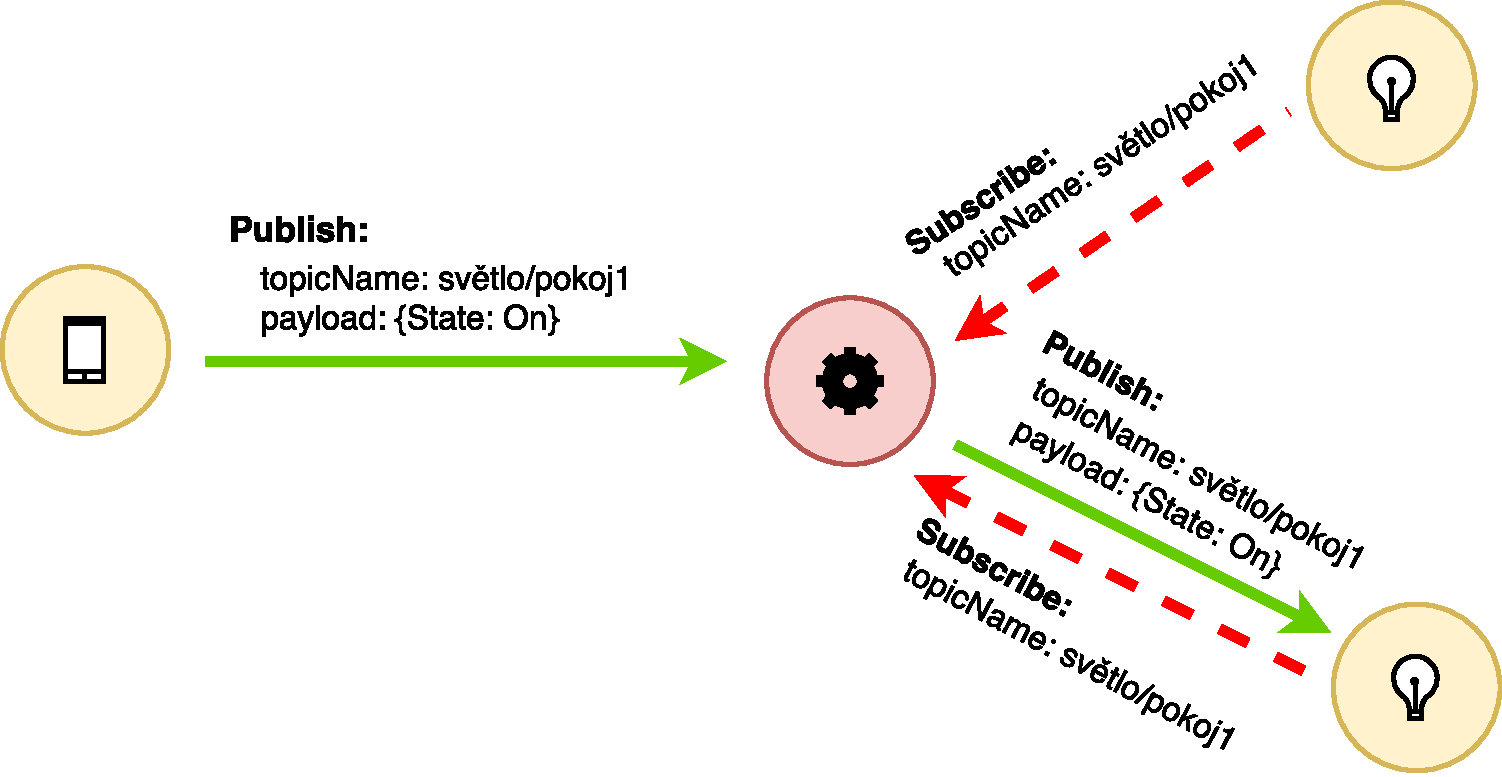
\includegraphics[scale=0.41]{pictures/mqtt-arch}
\caption{MQTT architektura}
\label{obr.mqtt-arch}
\end{center}
\end{figure}
  
  Další užitečnou položkou protokolu MQTT je QoS (Quality of Service),
  která může nabývat hodnot 0, 1 nebo 2.
  
   \begin{itemize}
    \item \textbf{QoS 0}
    
    Veškeré zprávy jsou odesílány bez potvrzení a žádným způsobem
    není zvýšena úroveň spolehlivosti, která je shodná se spolehlivostí protokolu TCP.
    
    \item \textbf{QoS 1}
    
    Pomocí potvrzování zajišťuje, že každá zpráva bude příjemci doručena alespoň jednou.
    
    \item \textbf{QoS 2}
    
     Umožňuje, aby každá zpráva byla spolehlivě doručena právě jednou.
   \end{itemize}
  Hodnota QoS se nastavuje vždy mezi dvěma uzly při navazování spojení.
  Z pohledu brokeru se může stát, že přijatá a odeslaná zpráva mají jiné QoS.
  Úrovně 1 a 2 dále umožňují perzistetní ukládání zpráv v případě, že příjemce je
  nedostupný. Zároveň platí, že s vyšší úrovní roste i režie komunikace. \cite{mqtt_intro}
 \subsubsection{Bezpečnost}
 Zabezpečení protokolu MQTT je možné rozdělit do následujících vrstev:
 \begin{itemize}
  \item \textbf{Síťová vrstva}
  
    Veškerá komunikace je postavena nad TCP/IP, a proto lze probíhající komunikaci
    zapouzdřit pomocí VPN připojení
    jako v běžných počítačových sítích. Kvůli větším nárokům na výkon je toto
    řešení vhodnější pro výkonější zařízení jako jsou například IoT brány, které
    mohou s brokerem navázat site-to-site spojení. \cite{mqtt_sec}
    
  \item \textbf{Transportní vrstva}
  
  Na této úrovni se využívá šifrování provozu pomocí protokolu TLS (Transport
  Layer Security). Omezením této metody jsou požadavky na výkon, které mohou být
  poměrně vysoké pokud nastává časté navazování spojení. \cite{mqtt_sec}
  
  \item \textbf{Aplikační vrstva}
  
  Samotný protokol MQTT nedefinuje žádné šifrovací mechanismy na aplikační úrovni. 
  Zabezpeční dat zde musí zajistit uživatel ještě před jejich zapouzdřením do MQTT zprávy. 
  Ovšem tímto způsobem je možné šifrovat jen tělo zprávy a hlavička zůstává nezměněná.
  
  Pro autentizaci je možné využít ověření pomocí jména a hesla nebo x.509 certifikátu.
  Jméno a heslo je přenášeno nešifrovaně, a proto je vhodné tuto metodu doplnit se 
  zabezpečením síťové nebo transportní vrstvy. Autentizaci pomocí certifikátů 
  je možné využít jen v případě použití TLS. Tato metoda je vhodnější pokud všechna
  zařízení jsou po jednotnou správou a je možné automatizovat distribuci 
  klientských certifikátů.
  
  Dále je na straně brokeru možné definovat pravidla pro autorizaci. Tyto pravidla 
  přiřazují klientů oprávnění pro provedení operací publish a subscribe
  nad příslušnými tématy. \cite{mqtt_sec}
  
 \end{itemize}

  \subsection{COAP}
  CoAP (Constrained Application Protocol) je otevřený přenosový protokol určený pro
  komunikaci síťových zařízení s velmi omezeným výkonem. Návrh vychází z RESTful
  (Representational State Transfer) principů, tudíž jeho použití je velmi vhodné
  v prostředích s již existujícím webových rozhraním, do kterého se snadno integruje. \cite{coap}
  
   \subsubsection{Způsob komunikace}
   Komunikace je postavena nad protokolem UDP (User Datagram Protocol) a vychází
   z modelu request/response, který se využívá u protokolu HTTP (Hypertext
   Transfer Protocol). Oproti protokolu HTTP je zde omezen počet možných operací
   a komunikace probíhá asynchronně. Dle důležitosti odesílané zprávy je možné určit,
   zda se má zasílat potvrzení či nikoli. Protože veškerá komunikace probíhá nad
   protokolem UDP, tak přenášené zprávy obsahují položku Message ID, která dokáže
   ošetřit duplikaci přijatých dat.
   %pokud to bude krátků můžu přidat option políčka pro udělání akce po splnění podmíky
   
   Pro zajištění integrace s běžnými webovými službami a zachování nízkých nároků
   se v CoAP topologii velmi často vyskytují proxy servery. Tyto servery mohou plnit
   funkci běžných reverzních a dopředných proxy, mapování mezi CoAP a HTTP protokolem
   nebo vyvažování zátěže. Způsob komunikace a schéma možné způsoby propojeí jsou na
   obrázku \ref{obr.coap-arch}. Senzor reprezentuje koncový prvek s omezeným výkonem.
   
   \begin{figure}[ht]
   \begin{center}
   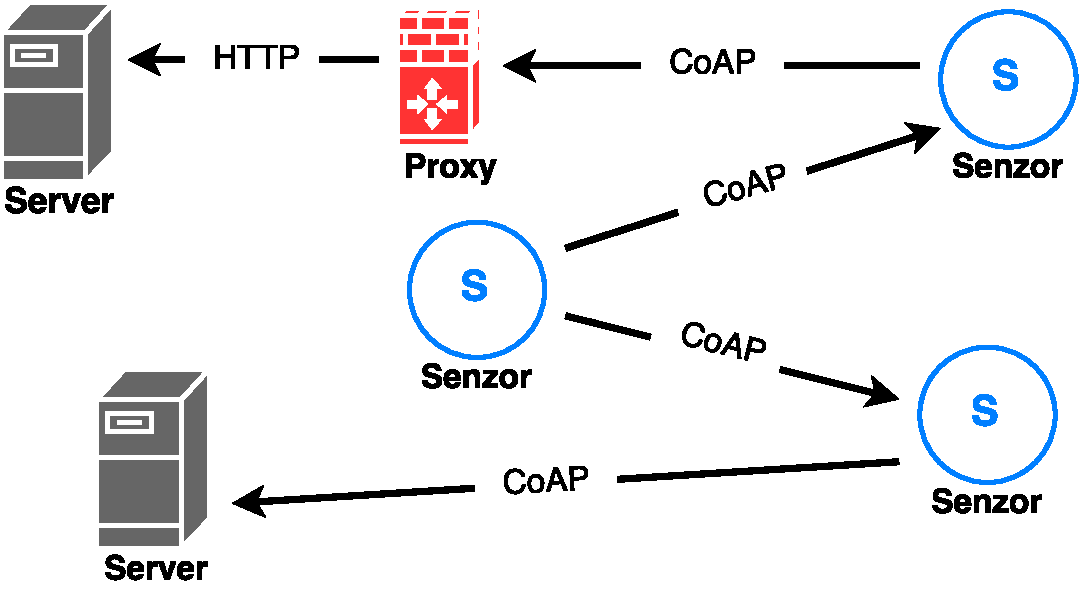
\includegraphics[scale=0.41]{pictures/coap-arch}
   \caption{CoAP architektura}
   \label{obr.coap-arch}
   \end{center}
   \end{figure}
   
   Ve specfikaci protokolu CoAP jsou definovány následující operace:
   \begin{itemize}
    \item \textbf{GET}
    
    Metoda \textit{GET} vrací aktuální stav požadovaného zdroje, který je identifikován pomocí
    URI (Uniform resource identifier). Tato operace je vždy bezpečná a idempotentní.
    
    \item \textbf{POST}
    
    \textit{POST} požadavek obsahuje ve svém těle novou reprezentaci cílového zdroje a požaduje 
    jeho zpracování. Funkce, která
    novou reprezentaci přijímá je definovaná na cílovém uzlu s příslušným URI.
    Výsledkem je vytvoření nového zdroje nebo aktualizace původního. Tato metoda
    není z pohledu zpracování bezpečná ani idempotentní.
    
    \item \textbf{PUT}
    
    Tato metoda specifikuje nový stav cílového zdroje, který specifikován použitým URI. Zdroj
    se buď vytvoří, nebo 
    v případě jeho existence aktualizuje. Provedení operace není bezpečné, ale 
    je idempotentní.
    
    \item \textbf{DELETE}
    
    Operace \textit{DELETE} požaduje smazání zdroje s příslušným URI. Tato metoda není bezpečná,
    ale je idempotentní.
    
   \end{itemize}
   
   Vyhledání potřebného zdroje je v topologii protokolu CoAP možné provést pomocí
   znalosti jeho URI nebo odesláním multicastového požadavku na definovanou
   skupinu uzlů. Možnost vyhledávání cílových zdrojů je velmi důležitá zejména
   v M2M prostředích. \cite{coap}
   
   \subsubsection{Bezpečnost}
   Samotný protokol nijak nedefinuje možnost autentizace a autorizace. V případě
   potřeby je nutné tyto mechanismy implementovat v aplikačním kódu. 
   
   Pro zajištění šifrování provozu nabízí CoAP následující režimy:
   \begin{itemize}
    \item \textbf{NoSec}
    
    Tento mód neobsahuje žádnou úroveň zabezpeční a veškeré zprávy jsou zasílány
    v otevřené podobě. 
    
    \item \textbf{PreSharedKey}
    
    V tomto případě se náváže spojení pomocí protokolu DTLS (Datagram Transport
    Layer Security), které využívá symetrické šifrování. Předsdílený klíč musí
    být známý všem uzlům před zahájením komunikace. 
    
    \item \textbf{RawPublicKey}
    
    Tento režim také navuzuje zabezpečené spojení pomocí protokolu DTLS, ale místo
    symetrické šifry se používá asymetrická.
    
    \item \textbf{Certificate}
    
    Mód \textit{Certificate} rozšiřuje \textit{RawPublicKey} o přidání certifikátu.
   \end{itemize}

   Podobně jako u protokolu MQTT je i zde možné ochránit provoz na síťové
   vrstvě pomocí VPN. Při nasazení libovolného režimu zabezpeční je nutné počítat 
   s většími nároky na výkon, které musí klient splňovat pro navazování a udržování 
   spojení. \cite{coap}
   
  \subsection{Z-Wave}
  
  Z-Wave je bezdrátový komunikační protokol určený pro senzorové sítě, který vysílá 
  v subgigahercových pásmech ISM (Industrial, Scientific and Medical). Veškeré komunikační
  prvky jsou certifikovány aliancí Z-Wave, která zároveň poskytuje technickou dokumentaci a
  licence pro vývoj. V současné době existují certifikace Z-Wave a Z-Wave Plus. 
  Z-Wave Plus zařízení obsahují nový chipset, který vylepšuje komunikační parametry
  sítě a zároveň je zpětně kompatibilní se staršími modely. \cite{z-plus}
  Otevřená implementace celého protokolu se nazývá OpenZWave \cite{openzwave}, která
  je vyvíjena komunitou. \cite{cesnet-survey} 
 
 \subsubsection{Způsob komunikace}
 V Z-Wave síti se může maximálně vyskytovat 232 uzlů, mezi kterými se vždy nachází jeden označený
 jako kontroler. Pro přidání libovolného zařízení do sítě musí být nejprve provedo příme spárování
 s kontrolerem. Během párovacího procesu nový prvek získá vlastní 8 bitový identifikátor (\textit{Node ID}) a 
 unikátní 32 bitový identifikátor sítě (\textit{Home ID}), který má již od výroby kontroler uložen v nepřepisovatelné paměti.
 Následné zasílání zpráv už nemusí probíhat přímo mezi senzorem a kontrolerem, ale zprávy mohou
 být přeposílány sousedními prvky, které jsou trvale napájené, čímž se velmi zvyšuje možná rozloha sítě. 
 Pro odebrání libolného zařízení je opět nutné zajisiti přimé spojení s kontrolerem a spustit odstraňovací
 proces. \cite{cesnet-survey}
 
 V rámci specifikace Z-Wave \cite{zwave-spec} je definován mechanismus pro určení dostupných příkazů. Každý senzor obsahuje
 svou definici tříd funkcionalit (\textit{Command Class}), které obsahují dostupné příkazy a formát odpovědi. Tyto definice
 jsou předány kontroleru během procesu párování. Příkladem může být třída \textit{Binary Switch}, která obsahuje příkazy:
 \begin{itemize}
 \item \textit{SET} - odesílá kontroler pro nastavení hodnoty 
 \item \textit{GET} - odesílá kontroler pro získání hodnoty  
 \item \textit{REPORT} - odesílá senzor jako odpověď na dotaz \textit{GET} 
 \end{itemize} 
 
 Při posílání zpráv je vždy vyžadováno potvrzení. V případě neobdržení potvrzení se vysílání opakuje. 
 Po třetím neúspěšném pokusu je požadavek zahozen.
 
 \subsubsection{Bezpečnost}
 Původní verze protokolu Z-Wave umožňovala volitelně využívat šifrování pomocí 128 bitového AES (Advanced Encryption Standard).
 Výměna symetrického klíče probíhá během počátečního párování, kde je vygenerovaný klíč šifrován pomocí výchozího
 klíče, který je uložen ve firmwaru. Vzhledem k tomuto postupu je dobré provádět počáteční párování na bezpečném
 místě, kde nemůže dojít k odposlechu. \cite{zwave-S0-attack}
 
 V roce 2016 Z-Wave aliance vydala nový S2 (Security 2) framework, který vylepšuje bezpečnostní funkcionality 
 a od roku 2017 je jeho použití povinné pro všechny nově certifikovaná zarízení. 
 
 S2 framework umožňuje zařízení rozdělit do následujících skupin s rozdílnými šifrovacími klíči:
 \begin{itemize}
  \item \textbf{Access Control} - 
   nejdůvěryhodnější třída, která obsahuje bezpečnostní prvky jako jsou například zámky,
   které zároveň podporují autentizaci
  \item \textbf{Authenticated} - 
  skupina určená pro běžné senzory, které podporují autentizaci 
  \item \textbf{Unauthenticated} - 
  třída pro ostatní prvky, které nepodporují autentizaci.
 \end{itemize}
 Autentizace probíhá pomocí PIN (Personal Identification Number) nebo QR (Quick Response) kódu.
 Výměna klíče je založena na algortmu ECDH (Elliptic-curve Diffie–Hellman), který zajišťuje 
 dostatečnou úroveň bezpečnosti během párovacího procesu. \cite{cesnet-survey}

 
  \subsection{BLE (Bluetooth Low Energy)} %!!! chybi citace
  BLE je bezdrátový prtokol určený pro senzorové sítě s důrazem na nízkou spotřebu. Byl představen 
  v roce 2010 jako součást specifikace Bluetooth 4.0 a je nekompatibilní s původními verzemi. 
  Za vývoj a údržbu protokolu je odpovědná skupina Bluetooth SIG (Special Interest Group).
  V současné době je nejnovější verzí Bluetooth 5.
  
  \subsubsection{Způsob komunikace}
  BLE vysílá v bezlicenčním ISM pásmu na frekvencích od 2.4 GHz do 2.4835 GHz. Specifikace
  protokolu vychází z Bluetooth, ale zejména díky změnám parametrů v rádiové vrstvě 
  jsou navzájem nekompatibilní. Do verze 4 umožňuje navázat pro koncová zařízení pouze jedno spojení,
  a proto 
  vytváří hvězdicovou topologii s jedním centrálním prvkem. Od verze 5 je možné využívat více připojení
  a lze vytvořit flexibilnější mesh topologii. 
  
  Před zahájením komunikace mezi centrálním prvkem a senzory je nutné nejprve prvést párování, 
  které probíhá v následujících krocích:
  \begin{itemize}
   \item \textbf{Vysílání žádostí}
   
   Při spuštění párování začně koncový prvek na kanálech určených pro propagaci všesměrově vysílat žádosti o připojení,
   které obsahují název zařízení, jméno výrobce a podporované služby.
   
   \item \textbf{Přijímání žádostí}
   
   Pokud je centrální prvek přepnutý do párovacího režimu, tak naslouchá příchozím požadavkům, které zobrazuje uživateli.
   Po výběru správného zařízení se ukončí mód naslouchání a začne se navazovat spojení.
   
   \item \textbf{Inicializace připojení} 
   
   Během této fáze se obě strany domlouvají na parametrech komunikace.
   \item \textbf{Komunikace}
   
   Po úspěšném navázání spojení je možná na základě dostupných služeb provádět zasílání zpráv.
  \end{itemize}

 
   \subsubsection{Bezpečnost}
   BLE umožňuje volitelně používat šifrování pomocí AES, jehož šifrovací klíč je 
   vytvořen behěm párování v části inicializace připojení. Velmi důležité je zabezpečit 
   výměnu sdíleného klíče, která až do verze 4.1 není bezpečná, protože neumožňuje ochranu
   před odposloucháváním. Vylepšení přichází až od verze 4.2, ve které lze využít ECDH.
   
   Vzhledem k různorodosti možných typů zařízení definuje BLE následující kategorie
   určující způsob výměny klíče:
    \begin{itemize}
     \item \textbf{Just Works}
     
     Nejjednodušší třída, která provádí výměnu automaticky a zároveň má nejmenší nároky 
     na připojované zařízení, které nemusí podporovat autentizaci. Díky chybějící autentizaci 
     je tato metoda zranitelná vůči MITM (Man in the middle) útokům.
     \item \textbf{Out of Band}
     
     V této kategorii jsou veškeré klíče vyměňovány odlišným komunikačním kanálem např. přes NFC (Near Field Communication).
     Celková bezpečnost této metody závisí na důvěryhodnoti použitého kanálu.
     \item \textbf{Passkey}
     
     Tato metoda vylepšuje \textit{Just Works} o autentizaci, která spočívá v uživatelském zadání šesti 
     místného kódu. Pro ochranu před odposlouchávání musí být použit algoritmus ECDH, který je dostupný
     až od verze 4.2.
     
     \item \textbf{Numeric Comparison}
     
     Využití tohoto způsobu párování je možné pouze od verze 4.2. Dochází zde k rozšíření metody \textit{Just Works}
     o jeden kontrolní krok, který slouží jako ochrana před MITM útokem. Po výměně klíčů každé zařízení
     vygeneruje šestimístný číselný kód, který následně zobrazí uživateli a čeká na jeho potvrzení.   
     
    \end{itemize}

   
   \newpage
 % popis a bezpečnostní analýza ZWave a Bluetooth
  \section{Bezpečnostní slabiny}
  Na základě provedené analýzy aktuálně používaných protokolů budou v této kapitole 
  popsány jejich bezpečnotní slabiny, které budou později využity při návrhu 
  detekčních algoritmů. Jelikož je tato práce zaměřena na senzorové protokoly 
  nekumunikující přes IP, budou v této kapitole popsány slabiny protokolů 
  Z-Wave a BLE.
  
 \subsection{Z-Wave}
 Hlavním problém jsou zařízení certifikovaná před březnem 2017, jelikož nepodporují S2 framework.
 Tyto prvky nemusí při své komunikaci využívat žádnou formu šifrování a síť se tak stává 
 velmi zranitelnou. V minulosti již bylo provedeno několik útoků, které pomocí projektu
 Scapy-Radio projektu \cite{ezwave} nebo knihovny OpenZWave  byly schnopny ovládat jednotlivé senzory. 
 %\cite{openzwave-attack}
 Při využití šifrování je velmi zranitelná doba během párovacího procesu, jelikož je při výměně
 šifrovacích klíčů použit výchozí klíč uložený ve firmware zařizení. Zároveň se 
 u jednoho typu zámku podařilo objevit implementační chybu \cite{zwave-S0-attack}, které umožňovala vnutit 
 nový šifrovací klíč a převzít tak kontrolu nad senzorem. 
 
 Při využití S2 frameworku dosud nebyly objeveny žádné zranitelnosti, ovšem tento
 framework je poměrně nový a většina používaných zařízení byla certifikována 
 ještě před jeho zavedením.
 
 \subsection{BLE}
 Velkou hrozbou jsou zařízení s verzí 4.1 nebo nižší, protože nepodporují žádnou ochranu před 
 odposlouchávání a MITM útokům v době párování. Od verze 4.2 je již pro výměnu klíčů použit ECDH 
 algoritmus, který zabraňuje možnému odposlouchávání, ale v případě použítí párovací metody, které
 nepodporuje autentizaci není zajištěna ochrana před MITM útoky.  \cite{cesnet-survey}
 
 Dalším problémem jsou samotní výrobci, kteří často nevyužívají bezpečnostní funkce protokolu  \cite{ble-locks} nebo
 implementují vlastní způsoby zabezpečení na aplikační úrovni. Tímto dochází k nezabepečení fáze 
 párování a často se vyskytují i implementační chyby, které přinášení další zranitelnosti \cite{ble-attack} a
 umožňují útočníkovi získat kontrolu nad celým provozem.  \cite{cesnet-survey}
 
 Nevýhodou je velmi dlouhá a komplikovaná specifikace protokolu, která vede k implementačním 
 chybám samotného BLE \cite{blueborne}. Tím vzniká nebezpečí, že i u výrobce, který využívá
 všech bezpečnostní funcionalit,
 se mohou vyskytovat zranitelnosti díky chybné implementaci komunikačních vrstev protokolu. \cite{cesnet-survey}
 
 \newpage
 \section{Možnosti detekce}
 V běžných IP sítích se pro detekci hrozeb nejčastěji používají IDS (Intrusion Detection System) a
 IPS (Intrustion Prevention System) systémy. Tyto služby rozšiřují koncept klasického firewallu, který
 blokuje nebo povoluje síťový provoz na základě statických pravidel, o podrobnější sledování 
 datových toků, které jsou zablokovány na základě nestandartního chování.
 
 IDS/IPS může být reprezentováno samostatným hardwarovým zařízením nebo softwarovým programem, který
 může být dále rozšířen o monitorovací sondy, které se starají pouze o sběr dat a jejich odesílání
 pro následnou analýzu. Zároveň
 se může lišit i umístění v síti. Detekční systémy lze provozovat před hraničním směrovačem 
 a detekovat tak kompletní příchozí a odchozí data nebo za hraničním směrovačem, což 
 umožní vyhodnocovat jen vyfiltrovaný provoz. Případně je možné nasadit IDS/IPS přímo na koncové
 stanice, kde kromě síťových dat lze získávat i informace o běhu systému. Poslední způsob poskytuje
 nejvíce detailní možnost analýzy, protože se provádí na míste vzniku komunikace a případný útok
 je možné zastavit již při jeho vzniku a zabránit případnému rozšíření. Nevýhodou takového nasazení
 je ztráta celkového pohledu na síť. Při zavedení IDS/IPS systému je z těchto důvodů dobré 
 kombinovat způsoby nasazení a umožnit vzájemné sdílení detekovaných incidentů.
 
 %\section{Metody zpracování}
 Při zaměření na zpracovávání datových toků lze dekteční systémy rozdělit do dvou základních kategorií:
 \begin{itemize}
  \item \textbf{Detekce anomálií}
  
  Tato metoda je založena na statistickém modelování. Nejprve se vytvoří profil běžného chování sítě, 
  který se následně porovnává s aktuálním provozem. Dle použité metody se může profil běžného provozu
  průběžně aktualizovat. Pokud měřené hodnoty síťového provozu překročí hodnotu stanoveného profilu
  nad definovaný limit, tak je detekován incident. Výhodou metody anomálií je její uplatnění i na 
  dosud neznámé útoky. Tento princip zároveň způsobuje větší míru falešných poplachů, a proto 
  je nutné jejich pečlivější ověření. Příkladem detekčních metod je: strojové učení, časové řady nebo
  stavové automaty \cite{ids-ips}.
  
  \item \textbf{Detekce signatur}
  
  V případě použítí této metody je využíváno signatur (profilů) předem známých útoků. Výhodou je, že díky 
  popsaným signaturám je tato metoda poměrně přesná a detekuje málo falešných incidentů. Naopak
  nevýhodou je, že není možné detekovat nové druhy útoků, pro které není známý profil. Problémem
  také je, že signatury musí být uloženy na nějakém perzistetním úložišti, které je dostupné 
  lokálně nebo vzdáleně \cite{ids-ips}.
 \end{itemize}
 
 %\section{Možnosti detekce}
 IoT sítě k běžnému IP provozu přidávají senzorové protokoly, jejichž chování je také dobré monitorovat, 
 protože jsou připojeny do počítačové sítě a mohou být zneužity při útocích. Bohužel detekční metody 
 nejsou pro tyto sítě moc rozšířené, a tím dochází ke zvýšení rizika a dopadu možných útoků. Pro určení 
 incidentů lze využít stejných principů jako v IP sítích, ale liší se způsob získávání dat pro analýzu. 
 Pro sběr informací lze využít následující přístupy:
 \begin{itemize}
  \item \textbf{Testbed}
  
    Tato metoda spočívá ve vytvoření specializovaného prostředí, ve kterém se nachází pouze testované 
    a měřící zařízení. Cílem je ověřit, že nově připojovaný senzor splňuje veškeré bezpečnostní 
    požadavky a neobsahuje žádné známe zranitelnosti. Měřící prvky reprezentují nástroje, které 
    jsou schopné odposlouchávat komunikaci a využívájí se také například při automatizovaných
    penetračních testech.   
  \item \textbf{Externí sonda}
  
  Funkce sondy je stejná jako v IP sítích. Jedná se o samostatné zařízení umístěné v sítí, které
  umožňuje sledovat probíhající komunikaci a odesílat získatné údaje ke zpracování. 
  Výhodou je velké množství, které lze získat, ale zároveň komplikací je šifrovaný provoz
  a často i cena kvalitní sondy.
  Dalším využitím 
  může být honeypot, kdy se sonda tváří jako zranitelný prvek a reportuje veškeré pokusy o útok.
    
  \item \textbf{Provozní statistiky}
  
  Posledním způsobem je sběr dat z příslušných rozhraní na IoT bráně. Tento postup nevyžaduje použití
  žádného dalšího zařízení, ale potřebuje, aby brána umožňovala získávat tyto statistiky. 
  Statistiky nejsou tak podrobné jako u externí sondy, ale výhodou je, 
  že získávání aktuálních dat o provozu je poměrně nenáročné.
 \end{itemize}
 
 Každá z předchozích metod používá jiný styl sběru dat. Při reálném použití je dobré vyhodnotit 
 bezpečnostní rizika a hrozby, podle kterých lze jednotlivé metody vhodně kombinovat.

 \newpage
 \section{Existující řešení}
 V součastnosti veškerá dostupná řešení se zaměřují na detekci útoků v IP protokolech. Mezi 
 současnými IDS/IPS existují signatury pouze pro SCADA (Supervisory Control And Data Acquisition)
 protokoly. Router Turris Omnia umožňuje nasadit systém Suricata, pro který nabízí rozšíření 
 PaKon \cite{pakon}. Toto rozšíření zpracovává data ze Suricaty, které následně ukládá v přehledné formě.
 Díky tomu užívatel získá podrovný přehled o stavu provozu. Získaná data může dále využívat 
 například k vylepšení stávajících bezpečnostních pravidel. Nevýhodou totoho řešení jsou 
 vyšší hardwarové požadavky, a proto ho nelze provozovat na branách s omezenými 
 prostředky. Další komplikací může být centralizovaná architektura a zameření pouze na 
 IP provoz.
 
 Na základě provedené analýzy nebylo nalezeno žadné řešení, které umožňuje vyhodnocovat 
 provoz aktuálně používaných IoT protoklů s ohledem na možné omezení hardwarových
 prostředků.
 
 \newpage
 \section{Analýza požadavků}
 Podstatnou částí návrhu výsledného řešení je přesné určení požadavků, které se dělí na 
 funkční a nefunkční. Funkční požadavky specifikují funkcionality kladené přímo na vznikající
 program, zatímco nefunkční spíše určují omezení vlastností systému a architekturu návrhu. V 
 následující kapitole budou popsány nároky na vznikají detekční nástroj, které vycházejí z obsahu
 zadání této práce a provedené analýzy.
 
  \subsection{Funkční požadavky}
  Kapitola popisuje funkční požadavky, které jsou od detekčního nástroje očekávány.
  \begin{itemize}
   \item \textbf{Sběr informací o provozu}
   
   Program bude umožňovat sběr dat na IoT bráně o aktuálním provozu z dostupných komunikačních
   rozhraní. Získané informace bude možné pomocí NEMEA \cite{nemea} (Network Measurements Analysis)
   frameworku předávat do dalších modulů.
   
   \item \textbf{Detekce anomálií}
   
   Vytvořený detekční algorimus bude schopen na základě získaných dat odhalit definované anomálie,
   které reprezentují neočekávané změny v síti. 
   
   \item \textbf{Konfigurace způsobu detekce}
   
   Detekční modul bude umožňovat nastavení parametrů pro jednotlivé zpracovávané položky
   pomocí konfiguračního souboru. Tyto 
   parametry budou následně sloužit jako vstup pro vytvořený detektor.
   
   \item \textbf{Zpracování získaných informací}
   
   Kromě analýzy dat a hlášení nalezených incidentů bude také možné zpracovaná data pravidelně 
   exportovat do dalších rozšiřujících modulů.
  \end{itemize}

  \subsection{Nefunkční požadavky}
  Kapitola obsahuje nefunkční požadavky, které jsou kladené na výsledný nástroj.
  \begin{itemize}
   \item \textbf{Rozšiřitelnost}
   
   Architektura celého řešení bude navržena tak, aby bylo možné rozšíření o nové 
   způsoby detekce anomálií a další typy provozních dat.
   
   \item \textbf{Flexibilita nasazení}
   
   Návrh způsobu detekce umožní fyzicky oddělit komponetu zajišťující sběr dat a komponetu vyhodnocující 
   provoz. Díky tomu bude možné provádět analýzu i na IoT branách s velmi omezeným prostředky, protože 
   tyto brány budou sloužit jako sondy, které budou posílat data do externího detektoru s dostatečnými 
   výkonem k provedení analýzy. 
   
   \item \textbf{Operační systém}
   
   Výsledné řešení bude implementováno a otestováno na operačním systému Ubuntu 16.04, na kterém 
   bude nasazena IoT brána BeeeOn a framework NEMEA. Zároveň
   budou při návrhu a implementaci vybírány takové technologie, aby bylo možné vytvořený program
   spustit pod distribuci OpenWrt, které je velmi rozšířena mezi síťovými prvky.   
  \end{itemize}

 \newpage 
 \section{Zvolené řešení}
 Obsahem této kapitoli je popis zvoleného řešení, které bylo na základě provedé analýzy
 určeno pro realizaci výsledného nástroje.
 
 Vytvořený detekční algorimus bude zaměřen na senzorové IoT protkoly, protože v současné době 
 neexistuje řešení, které by to umožňovalo. Pro analýzu budou použity protokoly Z-Wave a BLE, 
 které jsou v dnešních sítích velmi rozšířené. Algoritmus bude umístěň přímo na IoT bráně, která 
 je ideálním místem, protože
 se náchází velmi blízko koncových zařízení a má dostatečný výkon k vyhodnocování provozu. 
 Konkrétně bude použita brána BeeeOn, protože v současné době 
 jako jediná umožňuje sběr provozních dat o senzorových protokolech. 
 
 Pro účely detekce budou sbírány jen informace dostupné z lokálních rozhraní brány. Toto řešení
 je z hlediska reálného nasazení nejpravděpodobnější. Zároveň bude umožňěno rozšíření i pro další
 způsoby získávání dat. 
 
 Vyhodnocování dat bude probíhat metodou detekce anomálií, která je vhodná pro statistickou povahu dat
 , má menší nároky na množství dostupných prostředků a umožňuje rozpoznat i neznámé útoky.
 
 Jako programovací jazyk bude použit C++, protože podporuje objektový přístup a
 úspornou implementaci na paměť i procesorový čas. Zároveň tento jazyk je použit i v bráně
 BeeeOn, tudíž bude usnadněna integrace. Pro zajištění flexibility a možnosti dalšího rozšiřování 
 bude využito systému NEMEA, který také podporuje jazyk C++. 
 

% povídání o nutnosti učení se a nestaci jen blokovani portu, ... 
